% These are the lecture notes for my CSCI360 course SPRING 2017
% at John Jay College of Criminal Justice. They are based largely on
% Schneier's Applied Cryptography.

% Feel free to edit these slides and use them for your own courses.
% HOWEVER DO NOT REMOVE THESE LINES!
% Email me at: awood [at] jjay.cuny.edu
% or at: awood [at] gradcenter.cuny.edu


\documentclass{beamer}

\usepackage{tikz}
\usetikzlibrary{calc}

\usepackage{forest}
\usepackage{verbatim}
\usepackage{color}
\usepackage{amsmath}
\usepackage{graphicx}
\usepackage{caption}



\setbeamertemplate{footline}[frame number]
\setbeamertemplate{navigation symbols}{} 

\newtheorem{thm}{Theorem}[section]
\newtheorem{lem}{Lemma}
\newtheorem{cl}{Claim}
\newtheorem{cor}{Corollary}[section]
\newtheorem{conj}{Conjecture}
\newtheorem{quest}{Question}
\newtheorem{defn}{Definition}[section]
\newtheorem{obs}{Observation}[section]
\newtheorem{exam}{Example}

\newcommand{\im}{\operatorname{im}}
\newcommand{\id}{\operatorname{id}}
\newcommand{\interior}{\operatorname{int}}
\newcommand{\bdry}{\operatorname{bdry}}
\newcommand{\<}{\langle}
\renewcommand{\>}{\rangle}
\newcommand{\Gab}{(G_\phi)^{ab}} 
\newcommand{\phibar}{\bar{\phi}}
\newcommand{\Z}{\mathbb{Z}}
\newcommand{\N}{\mathbb{N}}
\newcommand{\Q}{\mathbb{Q}}
\newcommand{\R}{\mathbb{R}}
\newcommand{\C}{\mathbb{C}}
\newcommand{\A}{\mathcal{A}}
\newcommand{\OO}{\mathcal{O}}
\newcommand{\UU}{\mathcal{U}}
\newcommand{\power}{2^{\{P_1, \cdots , P_n\}}}
\newcommand{\bp}{\begin{problem}}
\newcommand{\ep}{\end{problem}}
\newcommand{\ba}{\begin{answer}}
\newcommand{\ea}{\end{answer}}
\newcommand{\ds}{\displaystyle}
\newcommand{\ben}{\renewcommand{\theenumi}{\alph{enumi}}
\renewcommand{\labelenumi}{(\theenumi)}\begin{enumerate}}
\newcommand{\een}{\end{enumerate}}
\newcommand{\Hess}{\operatorname{Hessian}}
\newcommand{\Aut}{\mathrm{Aut}}
\newcommand{\Inn}{\mathrm{Inn}}
\newcommand{\Out}{\mathrm{Out}}
\newcommand{\End}{\mathrm{End}}


\mode<presentation>
{
%  \usetheme{default}
  \setbeamercovered{invisible}
}


\usepackage[english]{babel}
\usepackage[latin1]{inputenc}
\usepackage{times}
\usepackage[T1]{fontenc}
\usepackage{stmaryrd}

%\usetheme{default}
%\usetheme{AnnArbor}
%\usetheme{Antibes}
%\usetheme{Bergen}
%\usetheme{Berkeley}
%\usetheme{Berlin}
%\usetheme{Boadilla}
%\usetheme{CambridgeUS}
%\usetheme{Copenhagen}
%\usetheme{Darmstadt}
%\usetheme{Dresden}
%\usetheme{Frankfurt}
%\usetheme{Goettingen}
%\usetheme{Hannover}
%\usetheme{Ilmenau}
%\usetheme{JuanLesPins}
%\usetheme{Luebeck}
%\usetheme{Madrid}
%\usetheme{Malmoe}
%\usetheme{Marburg}
%\usetheme{Montpellier}
%\usetheme{PaloAlto}
%\usetheme{Pittsburgh}
%\usetheme{Rochester}
\usetheme{Singapore}
%\usetheme{Szeged}
%\usetheme{Warsaw}

%\usecolortheme{default}
%\usecolortheme{albatross}
\usecolortheme{beaver}
%\usecolortheme{beetle}
%\usecolortheme{crane}
%\usecolortheme{dolphin}
%\usecolortheme{dove} % grey, white, yellow
%\usecolortheme{fly} %grey, yellow
%\usecolortheme{lily} %white, yellow, blue
%\usecolortheme{orchid}
%\usecolortheme{rose}
%\usecolortheme{seagull}
%\usecolortheme{seahorse}
%\usecolortheme{whale}
%\usecolortheme{wolverine}

% Title page

\title[DES]{History Of The Data Encryption Standard (DES)}

\subtitle{Based on \emph{Applied Cryptography} by Schneier, Chapter 12}

\author
{Lecture notes of Alexander Wood \\ \scriptsize \href{mailto:awood@jjay.cuny.edu}{awood@jjay.cuny.edu}}
\institute[JJay]{John Jay College of Criminal Justice}  

\date{}

\begin{document}

% Remove 'figure' text from figure captions 
\setbeamertemplate{caption}{\raggedright\insertcaption\par}

\begin{frame}
  \titlepage
\end{frame}


\section{History}

\begin{frame}
\frametitle{The DES}

The \textbf{Data Encryption Standard (DES)} is a private-key algorithm for encryption. It was developed in the 1970s and remained a worldwide standard for over 20 years after its publication.
\end{frame}


\begin{frame}
\frametitle{Early 1970s: Haphazard Cryptography}

Back in the early 1970s, the NSA was not even admitting their existence. The military had their own private communication methods, and several companies sold cryptographic equipment -- but the encryption methods were not public. 
\end{frame}


\begin{frame}
\frametitle{Kerckhoff's Principle}

Recall Kerckhoff's Principle, which states that \emph{the details of the cryptosystem should be able to be shared publicly} without compromising security.  \newline

However, details about the commercial encryption methods at the time were not available. 
\end{frame}


\begin{frame}
\frametitle{The Search For An Encryption Standard}

\begin{figure}
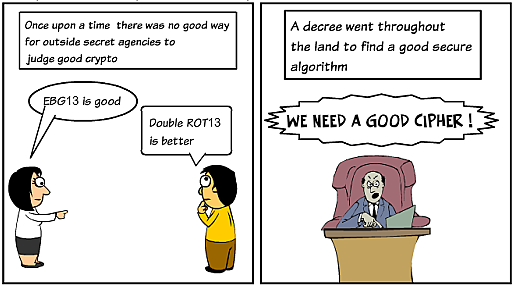
\includegraphics[scale=.7]{IMG/needacipher}
\end{figure}
{\scriptsize Image from: \url{https://www.howtogeek.com/howto/33949/htg-explains-what-is-encryption-and-how-does-it-work/}}
\end{frame}


\begin{frame}
\frametitle{The Search for an Encryption Standard}

\begin{figure}
\centering
\begin{minipage}{.5\textwidth}
  \centering
  
\includegraphics[width=.6\linewidth]{IMG/nbs}
  \label{fig:test1}
\end{minipage}%
\begin{minipage}{.5\textwidth}
  \centering
  
\includegraphics[width=.7\linewidth]{IMG/nist}
  \label{fig:test2}
\end{minipage}
\end{figure}

\emph{1972}: The National Bureau of Standards, now called the \textbf{National Institute for Standards and Technology (NIST)}, requested proposals for a cryptographic algorithm which could be put to standard use by the public. 
\end{frame}


\begin{frame}
\frametitle{NIST's Design Criteria}

NIST provided the following design criteria:\footnotesize

\begin{itemize}
\item The algorithm must provide a high level of security.
\item The algorithm must be \textbf{completely specified} and easy to understand.
\item The \textbf{security of the algorithm must reside in the key}; the security should not depend on the
secrecy of the algorithm. {\color{red}\textbf{$\leftarrow$ \emph{Kerckhoff's Principle!!!!}}}
\item The algorithm must be \textbf{available to all users}.
\item The algorithm must be adaptable for use in diverse applications.
\item The algorithm must be economically implementable in electronic devices.
\item The algorithm must be \textbf{efficient} to use.
\item The algorithm must be \textbf{able to be validated}.
\item The algorithm must be exportable.
\end{itemize}
\end{frame}


\begin{frame}
\frametitle{Cryptographic Standard: The Search Is On!}

Many ideas were proposed, but it took a while to find one which truly satisfied security requirements. 
\end{frame}

\begin{frame}
\frametitle{The Search Ends With... Lucifer}
\begin{columns}
\begin{column}{.5\textwidth}
During the early 1970's, researchers at IBM created a symmetric-key cipher called \textbf{Lucifer}, now known as the \textbf{Feistel cipher}.
\end{column}

\begin{column}{.5\textwidth}
\begin{figure}
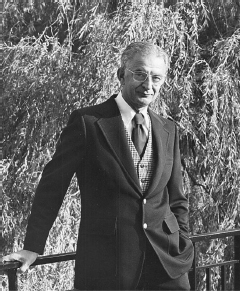
\includegraphics[scale=2]{IMG/feistel.jpg}
\caption{\scriptsize Horst Feistel}
\end{figure}
\end{column}
\end{columns}
\end{frame}


\begin{frame}
\frametitle{Publication of the DES}

\begin{figure}
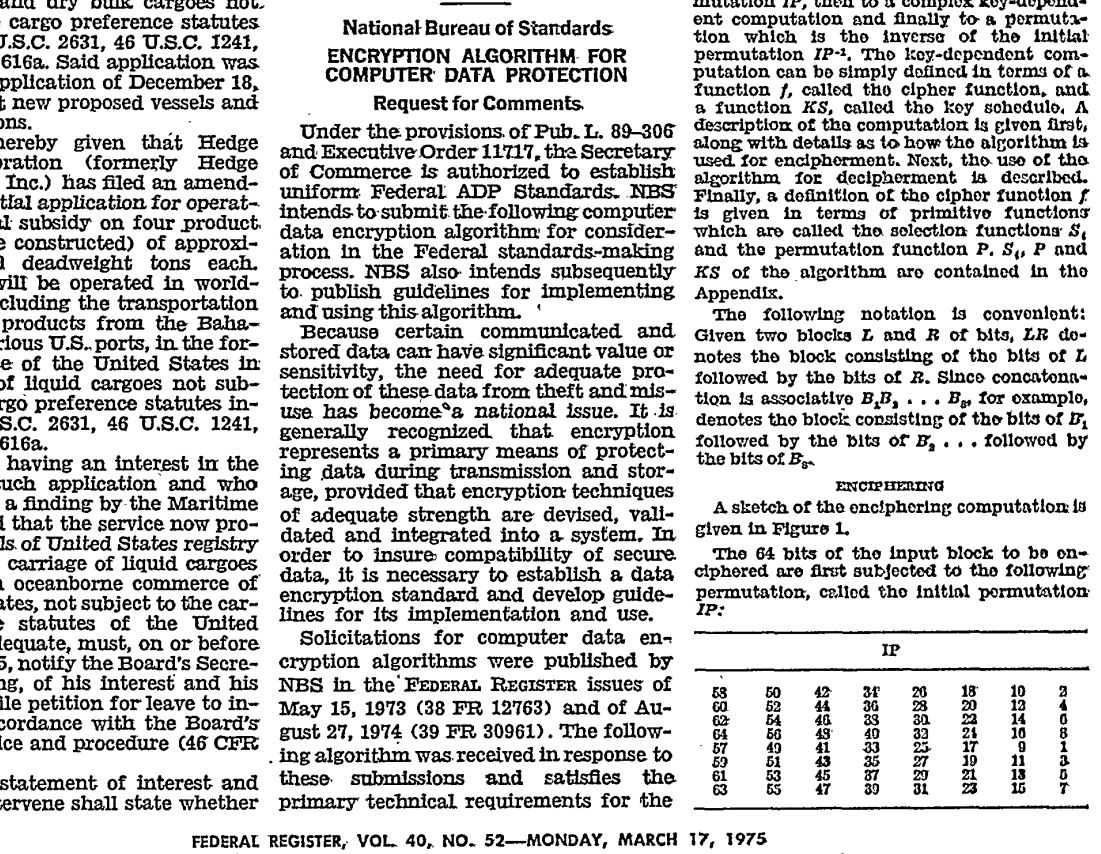
\includegraphics[scale=.4]{IMG/pub}
\end{figure}\small
NIST, IBM, and the NSA teamed up to evaluate the algorithm's security and suitability. Eventually in 1975 a modifed version of the algorithm was published in the \emph{Federal Register} on March 17, 1975. 
\end{frame}


\begin{frame}
\frametitle{Backdoor Controversy}

\begin{columns}
\begin{column}{.5\textwidth}
\begin{figure}
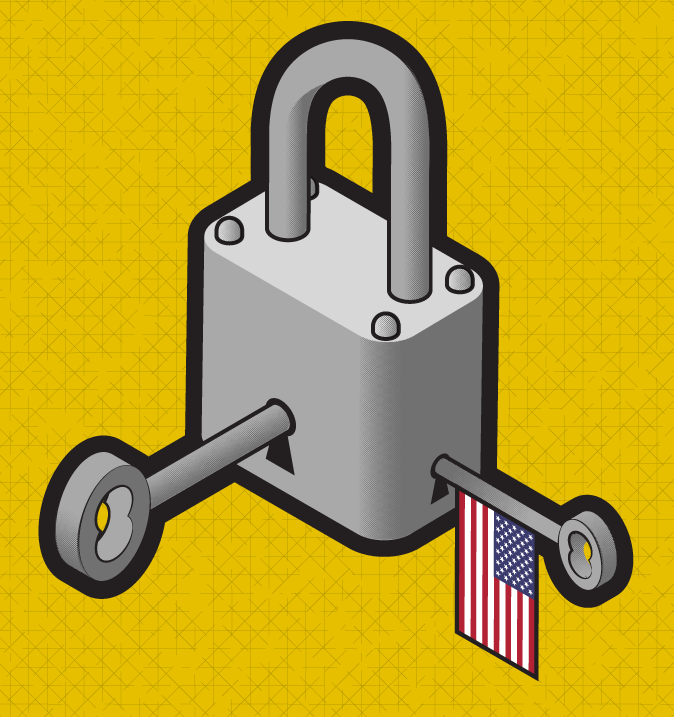
\includegraphics[scale=.2]{IMG/backdoor}
\caption{\scalebox{.4}{\url{http://www.vocativ.com/297409/presidential-candidate-encryption/}}}
\end{figure}
\end{column}

\begin{column}{.5\textwidth}\small
People were concerned that the NSA had included a ``backdoor'' in the DES.
\newline

A \textbf{backdoor} secret method by which a cryptographic system can be bypassed in order to obtain access to the plaintext of an encrypted message. \newline

Discussions about government backdoors and surveillance are increasingly relevant with current-day encryption. 
\end{column}
\end{columns}
\end{frame}

\begin{frame}
\frametitle{Backdoor Controversy: Key Length}

The controversy was rooted in the fact that the key length used in DES is only $56$ bits. \newline

Even before the DES was officially adopted as a standard, many asserted that this key length was too short -- and suspected that it had purposely been designed that way by the NSA.
\end{frame}



\begin{frame}
\frametitle{1977: Diffie and Hellman's Brute-Force Attack}


\begin{columns}
\begin{column}{.6\textwidth}
\begin{figure}
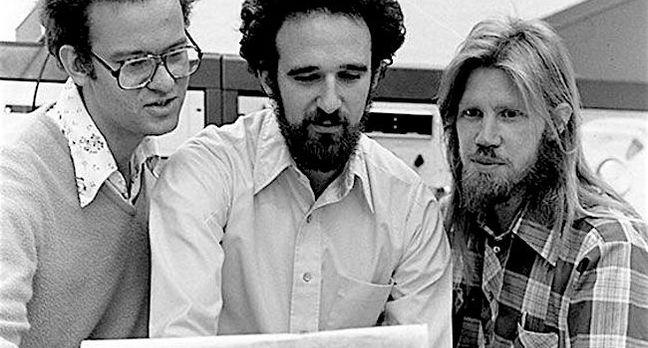
\includegraphics[scale=.3]{IMG/merkle_diffie_hellman}
\caption{\scriptsize Merkle, Diffie, and Hellman in 1977}
\end{figure}
\end{column}

\begin{column}{.4\textwidth}\small
Diffie and Hellman proposed a \$20 million dollar machine in 1977 which would be able to recover a DES key in one day. It exploited the small key length used by DES.
\end{column}
\end{columns}
\end{frame}



\begin{frame}
\frametitle{1993: Wiener's Brute-Force Attack}

In 1993, Michael Wiener designed a machine exploiting the short key length which, when built with 5760 chips, could be made for \$100K and find a DES key in 1.5 days. When built with 57600 chips the cost would be \$1 million but the DES key could be recovered in 3.5 hours. \newline

Neither Diffie and Hellman's machine nor Wiener's machine are known to have been made, but they showed that the DES could potentially be comprimised by even a brute-force attack.
\end{frame}







\section{Adoption}


\begin{frame}
\frametitle{1976: Adoption As Federal Standard}

\begin{figure}

\includegraphics[scale=.9]{IMG/commerce}
\end{figure}

The DES was adopted as a Federal Information Processing Standard (FIPS) on November 23, 1976 by the Secretary of Commerce. The official description of the standard was published in 1977. The DES was authorized for use for unclassified government communications. \newline
\end{frame}


\begin{frame}
\frametitle{The NSA's Regrets}
The DES was the first NSA-evaluated algorithm to be made public. It is speculated that this was on accident -- the NSA believed the DES was hardware-only and did not realize that NIST would publish enough information for the public to develop their own cryptographically secure software.\newline

The NSA claims off the record that publishing the DES was one of their biggest mistakes. Future algorithms remained classified. 
\end{frame}



\begin{frame}
\frametitle{1981: Adoption as a Private-Sector Standard}

\begin{figure}

\includegraphics[scale=.5]{IMG/ansi}
\end{figure}

In 1981 the American National Standards Institute (ANSI) approved DES as a standard in the private sector and published their own standard for modes of operation. Within ANSI, groups represented retail and banking developed their own standards based off of DES. 
\end{frame}

\begin{frame}
\frametitle{1992-1998: Time Marches On}

There was still not an alternative to the DES in 1992. It was recertified by NIST to remain the standard until 1998, and in 1997 a formal request was issued to search for alternatives during those years -- as it was suspected that the ``lifetime'' of the DES would end by the late 1990s.
\end{frame}



\begin{frame}
\frametitle{Rivest's Contests}

\begin{columns}
\begin{column}{.3\textwidth}
\begin{figure}
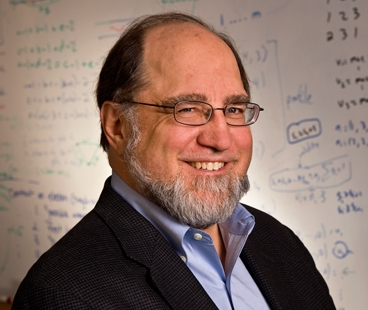
\includegraphics[scale=.28]{IMG/rivest}
\caption{\scriptsize Ronald Rivest}
\end{figure}
\end{column}

\begin{column}{.67\textwidth}\small
Ronald Rivest (the `R' of `RSA') funded four contests to break a DES encrypted message.
\begin{enumerate}[(Contest 1)]
\item 1996, broken in 96 days using distributed networks
\item 1997, broken in 41 days
\item 1998, broken in 56 hours using the Deep Crack computer
\item 1999, broken in 22 hours 15 minutes using Distributed Net and the EFF machine
\end{enumerate}
\end{column}
\end{columns}
\end{frame}


\begin{frame}
\frametitle{2001: Selection of AES Algorithm}

After announcing their intention to find a successor for DES in 1997, NIST selected an algorithm designed by Belgian cryptographers Joan Daemen and Vincent Rijmen called \textbf{Rijndael}. \newline

This cipher was modified and re-named the \textbf{Advanced Encryption Standard (AES)}, the chosen successor to DES.
\end{frame}



\begin{frame}
\frametitle{2005: DES Officially Withdrawn}

The DES was officially withdrawn in 2005. Triple DES, or \textbf{3DES}, is approved for sensitive government communication through 2030.\newline

3DES applies three iterations of DES which increases the key length to 168 bits. Meet-in-the-middle attacks reduce the level of effective security which 3DES can offer to 112 bits. 
\end{frame}



\begin{frame}
\frametitle{The Legacy of DES}

The DES has reached the end of its useful lifetime. However, the DES was the first cryptosystem of its caliber to have its algorithms made public. \newline

This revitalized the academic study of cryptography and spurred the development of modern cryptography as it is known today. 
\end{frame}


\begin{frame}
\frametitle{References}

\begin{itemize}
\item \emph{Applied Cryptography} By Schneier, Chapter 12
\item {\scriptsize\url{https://www.howtogeek.com/howto/33949/htg-explains-what-is-encryption-and-how-does-it-work/}}
\item {\scriptsize\url{http://searchsecurity.techtarget.com/definition/Data-Encryption-Standard}}
\item {\scriptsize\url{http://www-math.ucdenver.edu/~wcherowi/courses/m5410/des.pdf}}
\end{itemize}
\end{frame}
\end{document}


